\documentclass{standalone}
\usepackage{tikz}
\usetikzlibrary{patterns, positioning}


\begin{document}
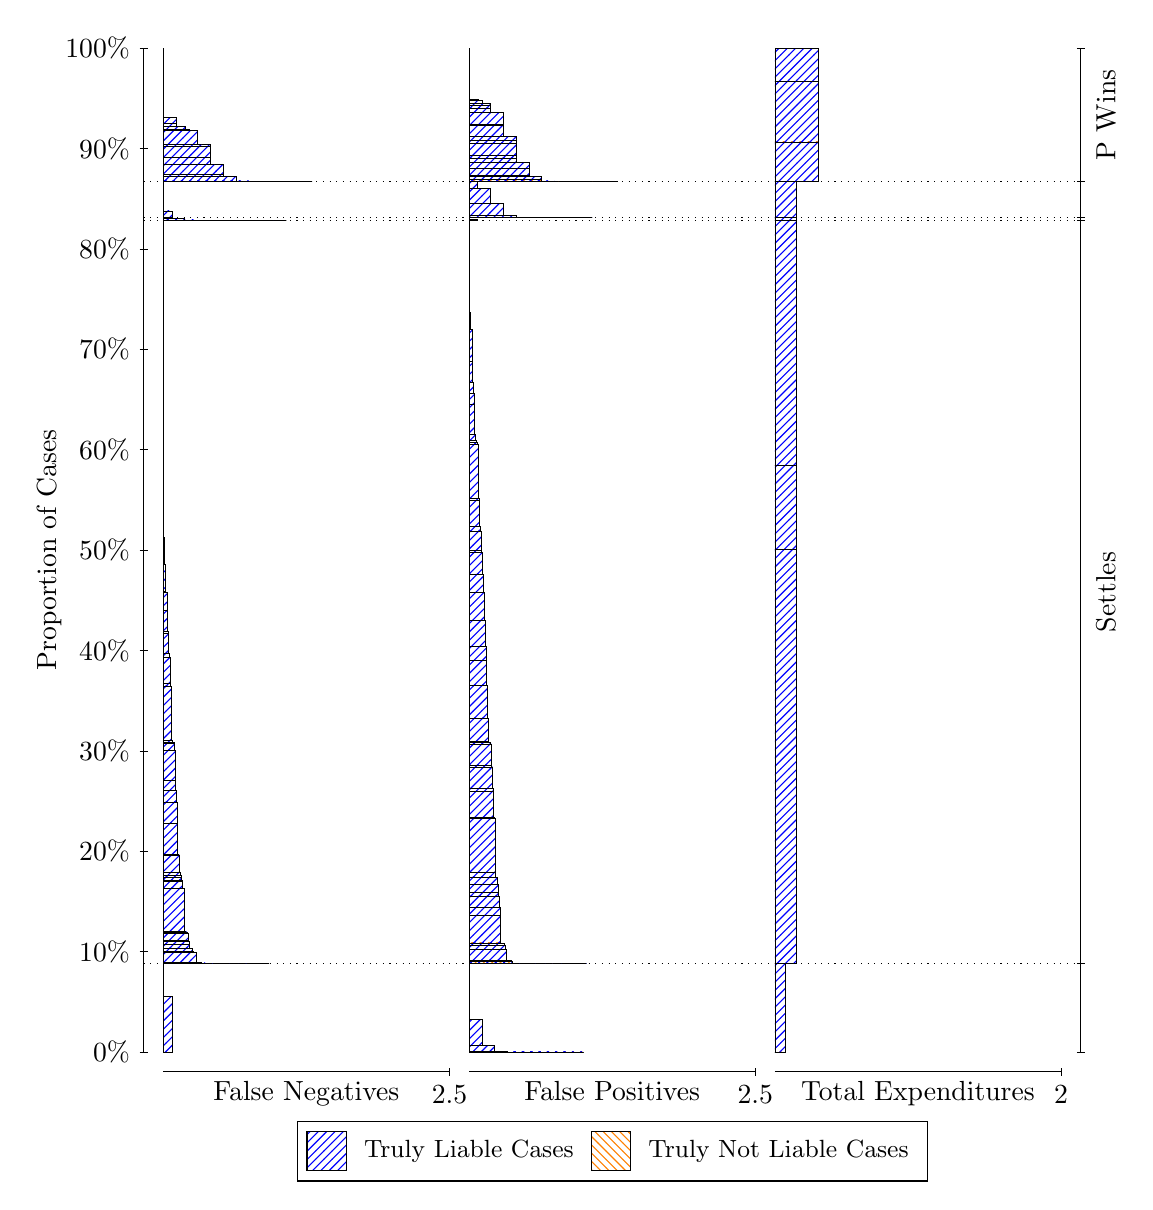
\begin{tikzpicture}
\draw[black, very thin] (1.5,1.75) -- (1.5,14.5);
\node[rotate=90, text=black, anchor=center] at (0.3, 8.125) {Proportion of Cases};
\draw[black, very thin] (1.45,1.75) -- (1.55,1.75);
\node[text=black, anchor=east] at (1.45, 1.75) {0\%};
\draw[black, very thin] (1.45,3.025) -- (1.55,3.025);
\node[text=black, anchor=east] at (1.45, 3.025) {10\%};
\draw[black, very thin] (1.45,4.3) -- (1.55,4.3);
\node[text=black, anchor=east] at (1.45, 4.3) {20\%};
\draw[black, very thin] (1.45,5.575) -- (1.55,5.575);
\node[text=black, anchor=east] at (1.45, 5.575) {30\%};
\draw[black, very thin] (1.45,6.85) -- (1.55,6.85);
\node[text=black, anchor=east] at (1.45, 6.85) {40\%};
\draw[black, very thin] (1.45,8.125) -- (1.55,8.125);
\node[text=black, anchor=east] at (1.45, 8.125) {50\%};
\draw[black, very thin] (1.45,9.4) -- (1.55,9.4);
\node[text=black, anchor=east] at (1.45, 9.4) {60\%};
\draw[black, very thin] (1.45,10.675) -- (1.55,10.675);
\node[text=black, anchor=east] at (1.45, 10.675) {70\%};
\draw[black, very thin] (1.45,11.95) -- (1.55,11.95);
\node[text=black, anchor=east] at (1.45, 11.95) {80\%};
\draw[black, very thin] (1.45,13.225) -- (1.55,13.225);
\node[text=black, anchor=east] at (1.45, 13.225) {90\%};
\draw[black, very thin] (1.45,14.5) -- (1.55,14.5);
\node[text=black, anchor=east] at (1.45, 14.5) {100\%};

\draw[black, very thin] (13.4,1.75) -- (13.4,14.5);
\draw[black, very thin] (13.35,1.75) -- (13.45,1.75);
\node[anchor=west] at (13.35, 1.75) {};
\draw[black, very thin] (13.35,2.8721) -- (13.45,2.8721);
\node[anchor=west] at (13.35, 2.8721) {};
\draw[black, very thin] (13.35,12.309) -- (13.45,12.309);
\node[anchor=west] at (13.35, 12.309) {};
\draw[black, very thin] (13.35,12.349) -- (13.45,12.349);
\node[anchor=west] at (13.35, 12.349) {};
\draw[black, very thin] (13.35,12.803) -- (13.45,12.803);
\node[anchor=west] at (13.35, 12.803) {};
\draw[black, very thin] (13.35,14.5) -- (13.45,14.5);
\node[anchor=west] at (13.35, 14.5) {};

\draw[black, very thin, pattern color=blue, pattern=north east lines] (1.75,1.75) rectangle (1.859,2.4561);
\draw[black, very thin, pattern color=orange, pattern=north west lines] (1.75,2.4561) rectangle (1.75,2.4561);
\draw[black, very thin, pattern color=blue, pattern=north east lines] (1.75,2.4561) rectangle (1.75,2.8721);
\draw[black, very thin, pattern color=blue, pattern=north east lines] (1.75,2.8721) rectangle (3.0943,2.8721);
\draw[black, very thin, pattern color=blue, pattern=north east lines] (1.75,2.8721) rectangle (3.0217,2.8721);
\draw[black, very thin, pattern color=blue, pattern=north east lines] (1.75,2.8721) rectangle (2.949,2.8721);
\draw[black, very thin, pattern color=blue, pattern=north east lines] (1.75,2.8721) rectangle (2.9329,2.8721);
\draw[black, very thin, pattern color=blue, pattern=north east lines] (1.75,2.8721) rectangle (2.8763,2.8721);
\draw[black, very thin, pattern color=blue, pattern=north east lines] (1.75,2.8721) rectangle (2.8602,2.8721);
\draw[black, very thin, pattern color=blue, pattern=north east lines] (1.75,2.8721) rectangle (2.8037,2.8721);
\draw[black, very thin, pattern color=blue, pattern=north east lines] (1.75,2.8721) rectangle (2.7875,2.8721);
\draw[black, very thin, pattern color=blue, pattern=north east lines] (1.75,2.8721) rectangle (2.7714,2.8721);
\draw[black, very thin, pattern color=blue, pattern=north east lines] (1.75,2.8721) rectangle (2.731,2.8721);
\draw[black, very thin, pattern color=blue, pattern=north east lines] (1.75,2.8721) rectangle (2.7149,2.8721);
\draw[black, very thin, pattern color=blue, pattern=north east lines] (1.75,2.8721) rectangle (2.6987,2.8721);
\draw[black, very thin, pattern color=blue, pattern=north east lines] (1.75,2.8721) rectangle (2.6583,2.8721);
\draw[black, very thin, pattern color=blue, pattern=north east lines] (1.75,2.8721) rectangle (2.6422,2.8721);
\draw[black, very thin, pattern color=blue, pattern=north east lines] (1.75,2.8721) rectangle (2.626,2.8721);
\draw[black, very thin, pattern color=blue, pattern=north east lines] (1.75,2.8721) rectangle (2.6099,2.8721);
\draw[black, very thin, pattern color=blue, pattern=north east lines] (1.75,2.8721) rectangle (2.5857,2.8721);
\draw[black, very thin, pattern color=blue, pattern=north east lines] (1.75,2.8721) rectangle (2.5695,2.8721);
\draw[black, very thin, pattern color=blue, pattern=north east lines] (1.75,2.8721) rectangle (2.5534,2.8721);
\draw[black, very thin, pattern color=blue, pattern=north east lines] (1.75,2.8721) rectangle (2.5372,2.8721);
\draw[black, very thin, pattern color=blue, pattern=north east lines] (1.75,2.8721) rectangle (2.513,2.8721);
\draw[black, very thin, pattern color=blue, pattern=north east lines] (1.75,2.8721) rectangle (2.4969,2.8721);
\draw[black, very thin, pattern color=blue, pattern=north east lines] (1.75,2.8721) rectangle (2.4807,2.8721);
\draw[black, very thin, pattern color=blue, pattern=north east lines] (1.75,2.8721) rectangle (2.4646,2.8721);
\draw[black, very thin, pattern color=blue, pattern=north east lines] (1.75,2.8721) rectangle (2.4484,2.8721);
\draw[black, very thin, pattern color=blue, pattern=north east lines] (1.75,2.8721) rectangle (2.4403,2.8722);
\draw[black, very thin, pattern color=blue, pattern=north east lines] (1.75,2.8722) rectangle (2.4242,2.8722);
\draw[black, very thin, pattern color=blue, pattern=north east lines] (1.75,2.8722) rectangle (2.408,2.8722);
\draw[black, very thin, pattern color=blue, pattern=north east lines] (1.75,2.8722) rectangle (2.3919,2.8722);
\draw[black, very thin, pattern color=blue, pattern=north east lines] (1.75,2.8722) rectangle (2.3757,2.8722);
\draw[black, very thin, pattern color=blue, pattern=north east lines] (1.75,2.8722) rectangle (2.3677,2.8722);
\draw[black, very thin, pattern color=blue, pattern=north east lines] (1.75,2.8722) rectangle (2.3677,2.8722);
\draw[black, very thin, pattern color=blue, pattern=north east lines] (1.75,2.8722) rectangle (2.3515,2.8722);
\draw[black, very thin, pattern color=blue, pattern=north east lines] (1.75,2.8722) rectangle (2.3354,2.8779);
\draw[black, very thin, pattern color=blue, pattern=north east lines] (1.75,2.8779) rectangle (2.3192,2.878);
\draw[black, very thin, pattern color=blue, pattern=north east lines] (1.75,2.878) rectangle (2.3031,2.878);
\draw[black, very thin, pattern color=blue, pattern=north east lines] (1.75,2.878) rectangle (2.295,2.8782);
\draw[black, very thin, pattern color=blue, pattern=north east lines] (1.75,2.8782) rectangle (2.2869,2.8782);
\draw[black, very thin, pattern color=blue, pattern=north east lines] (1.75,2.8782) rectangle (2.2789,2.8805);
\draw[black, very thin, pattern color=blue, pattern=north east lines] (1.75,2.8805) rectangle (2.2627,2.8805);
\draw[black, very thin, pattern color=blue, pattern=north east lines] (1.75,2.8805) rectangle (2.2466,2.8828);
\draw[black, very thin, pattern color=blue, pattern=north east lines] (1.75,2.8828) rectangle (2.2304,2.8831);
\draw[black, very thin, pattern color=blue, pattern=north east lines] (1.75,2.8831) rectangle (2.2223,2.8909);
\draw[black, very thin, pattern color=blue, pattern=north east lines] (1.75,2.8909) rectangle (2.2143,2.8909);
\draw[black, very thin, pattern color=blue, pattern=north east lines] (1.75,2.8909) rectangle (2.2062,2.8909);
\draw[black, very thin, pattern color=blue, pattern=north east lines] (1.75,2.8909) rectangle (2.2062,2.8913);
\draw[black, very thin, pattern color=blue, pattern=north east lines] (1.75,2.8913) rectangle (2.19,2.8915);
\draw[black, very thin, pattern color=blue, pattern=north east lines] (1.75,2.8915) rectangle (2.1739,3.0104);
\draw[black, very thin, pattern color=blue, pattern=north east lines] (1.75,3.0104) rectangle (2.1577,3.0161);
\draw[black, very thin, pattern color=blue, pattern=north east lines] (1.75,3.0161) rectangle (2.1497,3.0179);
\draw[black, very thin, pattern color=blue, pattern=north east lines] (1.75,3.0179) rectangle (2.1416,3.0187);
\draw[black, very thin, pattern color=blue, pattern=north east lines] (1.75,3.0187) rectangle (2.1335,3.0222);
\draw[black, very thin, pattern color=blue, pattern=north east lines] (1.75,3.0222) rectangle (2.1254,3.0235);
\draw[black, very thin, pattern color=blue, pattern=north east lines] (1.75,3.0235) rectangle (2.1174,3.0705);
\draw[black, very thin, pattern color=blue, pattern=north east lines] (1.75,3.0705) rectangle (2.1012,3.0706);
\draw[black, very thin, pattern color=blue, pattern=north east lines] (1.75,3.0706) rectangle (2.0851,3.1236);
\draw[black, very thin, pattern color=blue, pattern=north east lines] (1.75,3.1236) rectangle (2.077,3.1586);
\draw[black, very thin, pattern color=blue, pattern=north east lines] (1.75,3.1586) rectangle (2.0689,3.1702);
\draw[black, very thin, pattern color=blue, pattern=north east lines] (1.75,3.1702) rectangle (2.0609,3.2631);
\draw[black, very thin, pattern color=blue, pattern=north east lines] (1.75,3.2631) rectangle (2.0528,3.2675);
\draw[black, very thin, pattern color=blue, pattern=north east lines] (1.75,3.2675) rectangle (2.0447,3.2676);
\draw[black, very thin, pattern color=blue, pattern=north east lines] (1.75,3.2676) rectangle (2.0447,3.2743);
\draw[black, very thin, pattern color=blue, pattern=north east lines] (1.75,3.2743) rectangle (2.0286,3.2787);
\draw[black, very thin, pattern color=blue, pattern=north east lines] (1.75,3.2787) rectangle (2.0124,3.8245);
\draw[black, very thin, pattern color=blue, pattern=north east lines] (1.75,3.8245) rectangle (2.0043,3.8328);
\draw[black, very thin, pattern color=blue, pattern=north east lines] (1.75,3.8328) rectangle (1.9963,3.9185);
\draw[black, very thin, pattern color=blue, pattern=north east lines] (1.75,3.9185) rectangle (1.9882,3.9366);
\draw[black, very thin, pattern color=blue, pattern=north east lines] (1.75,3.9366) rectangle (1.9801,3.9731);
\draw[black, very thin, pattern color=blue, pattern=north east lines] (1.75,3.9731) rectangle (1.972,3.9939);
\draw[black, very thin, pattern color=blue, pattern=north east lines] (1.75,3.9939) rectangle (1.964,4.0312);
\draw[black, very thin, pattern color=blue, pattern=north east lines] (1.75,4.0312) rectangle (1.9559,4.2534);
\draw[black, very thin, pattern color=blue, pattern=north east lines] (1.75,4.2534) rectangle (1.9397,4.2556);
\draw[black, very thin, pattern color=blue, pattern=north east lines] (1.75,4.2556) rectangle (1.9317,4.6583);
\draw[black, very thin, pattern color=blue, pattern=north east lines] (1.75,4.6583) rectangle (1.9236,4.9253);
\draw[black, very thin, pattern color=blue, pattern=north east lines] (1.75,4.9253) rectangle (1.9155,5.0698);
\draw[black, very thin, pattern color=blue, pattern=north east lines] (1.75,5.0698) rectangle (1.9074,5.2025);
\draw[black, very thin, pattern color=blue, pattern=north east lines] (1.75,5.2025) rectangle (1.8994,5.5858);
\draw[black, very thin, pattern color=blue, pattern=north east lines] (1.75,5.5858) rectangle (1.8913,5.6665);
\draw[black, very thin, pattern color=blue, pattern=north east lines] (1.75,5.6665) rectangle (1.8832,5.667);
\draw[black, very thin, pattern color=blue, pattern=north east lines] (1.75,5.667) rectangle (1.8832,5.686);
\draw[black, very thin, pattern color=blue, pattern=north east lines] (1.75,5.686) rectangle (1.8671,5.7085);
\draw[black, very thin, pattern color=blue, pattern=north east lines] (1.75,5.7085) rectangle (1.8509,6.399);
\draw[black, very thin, pattern color=blue, pattern=north east lines] (1.75,6.399) rectangle (1.8429,6.4278);
\draw[black, very thin, pattern color=blue, pattern=north east lines] (1.75,6.4278) rectangle (1.8348,6.7572);
\draw[black, very thin, pattern color=blue, pattern=north east lines] (1.75,6.7572) rectangle (1.8267,6.812);
\draw[black, very thin, pattern color=blue, pattern=north east lines] (1.75,6.812) rectangle (1.8186,7.0636);
\draw[black, very thin, pattern color=blue, pattern=north east lines] (1.75,7.0636) rectangle (1.8106,7.087);
\draw[black, very thin, pattern color=blue, pattern=north east lines] (1.75,7.087) rectangle (1.8025,7.3588);
\draw[black, very thin, pattern color=blue, pattern=north east lines] (1.75,7.3588) rectangle (1.7944,7.5907);
\draw[black, very thin, pattern color=blue, pattern=north east lines] (1.75,7.5907) rectangle (1.7783,7.5957);
\draw[black, very thin, pattern color=blue, pattern=north east lines] (1.75,7.5957) rectangle (1.7702,7.9459);
\draw[black, very thin, pattern color=blue, pattern=north east lines] (1.75,7.9459) rectangle (1.7621,8.2807);
\draw[black, very thin, pattern color=blue, pattern=north east lines] (1.75,8.2807) rectangle (1.754,8.4584);
\draw[black, very thin, pattern color=orange, pattern=north west lines] (1.75,8.4584) rectangle (1.75,8.4584);
\draw[black, very thin, pattern color=blue, pattern=north east lines] (1.75,8.4584) rectangle (1.75,12.309);
\draw[black, very thin, pattern color=blue, pattern=north east lines] (1.75,12.309) rectangle (3.3123,12.309);
\draw[black, very thin, pattern color=blue, pattern=north east lines] (1.75,12.309) rectangle (3.1509,12.309);
\draw[black, very thin, pattern color=blue, pattern=north east lines] (1.75,12.309) rectangle (2.9894,12.309);
\draw[black, very thin, pattern color=blue, pattern=north east lines] (1.75,12.309) rectangle (2.8279,12.309);
\draw[black, very thin, pattern color=blue, pattern=north east lines] (1.75,12.309) rectangle (2.6664,12.309);
\draw[black, very thin, pattern color=blue, pattern=north east lines] (1.75,12.309) rectangle (2.5049,12.309);
\draw[black, very thin, pattern color=blue, pattern=north east lines] (1.75,12.309) rectangle (2.3434,12.31);
\draw[black, very thin, pattern color=blue, pattern=north east lines] (1.75,12.31) rectangle (2.182,12.318);
\draw[black, very thin, pattern color=blue, pattern=north east lines] (1.75,12.318) rectangle (2.0205,12.337);
\draw[black, very thin, pattern color=blue, pattern=north east lines] (1.75,12.337) rectangle (1.859,12.349);
\draw[black, very thin, pattern color=orange, pattern=north west lines] (1.75,12.349) rectangle (1.75,12.349);
\draw[black, very thin, pattern color=blue, pattern=north east lines] (1.75,12.349) rectangle (1.859,12.431);
\draw[black, very thin, pattern color=orange, pattern=north west lines] (1.75,12.431) rectangle (1.75,12.431);
\draw[black, very thin, pattern color=blue, pattern=north east lines] (1.75,12.431) rectangle (1.75,12.803);
\draw[black, very thin, pattern color=blue, pattern=north east lines] (1.75,12.803) rectangle (3.6393,12.803);
\draw[black, very thin, pattern color=blue, pattern=north east lines] (1.75,12.803) rectangle (3.4779,12.803);
\draw[black, very thin, pattern color=blue, pattern=north east lines] (1.75,12.803) rectangle (3.3164,12.803);
\draw[black, very thin, pattern color=blue, pattern=north east lines] (1.75,12.803) rectangle (3.1549,12.803);
\draw[black, very thin, pattern color=blue, pattern=north east lines] (1.75,12.803) rectangle (3.1549,12.803);
\draw[black, very thin, pattern color=blue, pattern=north east lines] (1.75,12.803) rectangle (2.9934,12.803);
\draw[black, very thin, pattern color=blue, pattern=north east lines] (1.75,12.803) rectangle (2.9934,12.804);
\draw[black, very thin, pattern color=blue, pattern=north east lines] (1.75,12.804) rectangle (2.8804,12.804);
\draw[black, very thin, pattern color=blue, pattern=north east lines] (1.75,12.804) rectangle (2.8319,12.814);
\draw[black, very thin, pattern color=blue, pattern=north east lines] (1.75,12.814) rectangle (2.7189,12.814);
\draw[black, very thin, pattern color=blue, pattern=north east lines] (1.75,12.814) rectangle (2.7189,12.814);
\draw[black, very thin, pattern color=blue, pattern=north east lines] (1.75,12.814) rectangle (2.6704,12.865);
\draw[black, very thin, pattern color=blue, pattern=north east lines] (1.75,12.865) rectangle (2.5574,12.865);
\draw[black, very thin, pattern color=blue, pattern=north east lines] (1.75,12.865) rectangle (2.509,12.896);
\draw[black, very thin, pattern color=blue, pattern=north east lines] (1.75,12.896) rectangle (2.509,13.024);
\draw[black, very thin, pattern color=blue, pattern=north east lines] (1.75,13.024) rectangle (2.3959,13.024);
\draw[black, very thin, pattern color=blue, pattern=north east lines] (1.75,13.024) rectangle (2.3959,13.024);
\draw[black, very thin, pattern color=blue, pattern=north east lines] (1.75,13.024) rectangle (2.3475,13.115);
\draw[black, very thin, pattern color=blue, pattern=north east lines] (1.75,13.115) rectangle (2.3475,13.253);
\draw[black, very thin, pattern color=blue, pattern=north east lines] (1.75,13.253) rectangle (2.3475,13.278);
\draw[black, very thin, pattern color=blue, pattern=north east lines] (1.75,13.278) rectangle (2.2344,13.278);
\draw[black, very thin, pattern color=blue, pattern=north east lines] (1.75,13.278) rectangle (2.2344,13.278);
\draw[black, very thin, pattern color=blue, pattern=north east lines] (1.75,13.278) rectangle (2.2344,13.278);
\draw[black, very thin, pattern color=blue, pattern=north east lines] (1.75,13.278) rectangle (2.186,13.456);
\draw[black, very thin, pattern color=blue, pattern=north east lines] (1.75,13.456) rectangle (2.073,13.456);
\draw[black, very thin, pattern color=blue, pattern=north east lines] (1.75,13.456) rectangle (2.073,13.468);
\draw[black, very thin, pattern color=blue, pattern=north east lines] (1.75,13.468) rectangle (2.0245,13.469);
\draw[black, very thin, pattern color=blue, pattern=north east lines] (1.75,13.469) rectangle (2.0245,13.509);
\draw[black, very thin, pattern color=blue, pattern=north east lines] (1.75,13.509) rectangle (2.0245,13.509);
\draw[black, very thin, pattern color=blue, pattern=north east lines] (1.75,13.509) rectangle (1.9115,13.539);
\draw[black, very thin, pattern color=blue, pattern=north east lines] (1.75,13.539) rectangle (1.9115,13.544);
\draw[black, very thin, pattern color=blue, pattern=north east lines] (1.75,13.544) rectangle (1.9115,13.619);
\draw[black, very thin, pattern color=blue, pattern=north east lines] (1.75,13.619) rectangle (1.863,13.62);
\draw[black, very thin, pattern color=blue, pattern=north east lines] (1.75,13.62) rectangle (1.863,13.62);
\draw[black, very thin, pattern color=orange, pattern=north west lines] (1.75,13.62) rectangle (1.75,13.62);
\draw[black, very thin, pattern color=blue, pattern=north east lines] (1.75,13.62) rectangle (1.75,14.5);
\draw[black, very thin, pattern color=orange, pattern=north west lines] (5.6333,1.75) rectangle (7.0867,1.75);
\draw[black, very thin, pattern color=blue, pattern=north east lines] (5.6333,1.75) rectangle (7.0867,1.75);
\draw[black, very thin, pattern color=blue, pattern=north east lines] (5.6333,1.75) rectangle (6.9252,1.75);
\draw[black, very thin, pattern color=blue, pattern=north east lines] (5.6333,1.75) rectangle (6.7637,1.75);
\draw[black, very thin, pattern color=blue, pattern=north east lines] (5.6333,1.75) rectangle (6.6022,1.75);
\draw[black, very thin, pattern color=blue, pattern=north east lines] (5.6333,1.75) rectangle (6.4407,1.75);
\draw[black, very thin, pattern color=blue, pattern=north east lines] (5.6333,1.75) rectangle (6.2793,1.7503);
\draw[black, very thin, pattern color=blue, pattern=north east lines] (5.6333,1.7503) rectangle (6.1178,1.7579);
\draw[black, very thin, pattern color=blue, pattern=north east lines] (5.6333,1.7579) rectangle (5.9563,1.8357);
\draw[black, very thin, pattern color=blue, pattern=north east lines] (5.6333,1.8357) rectangle (5.7948,2.166);
\draw[black, very thin, pattern color=blue, pattern=north east lines] (5.6333,2.166) rectangle (5.6333,2.8721);
\draw[black, very thin, pattern color=orange, pattern=north west lines] (5.6333,2.8721) rectangle (7.123,2.8721);
\draw[black, very thin, pattern color=blue, pattern=north east lines] (5.6333,2.8721) rectangle (7.123,2.8721);
\draw[black, very thin, pattern color=orange, pattern=north west lines] (5.6333,2.8721) rectangle (7.0503,2.8721);
\draw[black, very thin, pattern color=blue, pattern=north east lines] (5.6333,2.8721) rectangle (7.0503,2.8721);
\draw[black, very thin, pattern color=orange, pattern=north west lines] (5.6333,2.8721) rectangle (6.9777,2.8721);
\draw[black, very thin, pattern color=blue, pattern=north east lines] (5.6333,2.8721) rectangle (6.9777,2.8721);
\draw[black, very thin, pattern color=blue, pattern=north east lines] (5.6333,2.8721) rectangle (6.9615,2.8721);
\draw[black, very thin, pattern color=orange, pattern=north west lines] (5.6333,2.8721) rectangle (6.905,2.8721);
\draw[black, very thin, pattern color=blue, pattern=north east lines] (5.6333,2.8721) rectangle (6.905,2.8721);
\draw[black, very thin, pattern color=blue, pattern=north east lines] (5.6333,2.8721) rectangle (6.8889,2.8721);
\draw[black, very thin, pattern color=orange, pattern=north west lines] (5.6333,2.8721) rectangle (6.8323,2.8721);
\draw[black, very thin, pattern color=blue, pattern=north east lines] (5.6333,2.8721) rectangle (6.8323,2.8721);
\draw[black, very thin, pattern color=blue, pattern=north east lines] (5.6333,2.8721) rectangle (6.8162,2.8721);
\draw[black, very thin, pattern color=blue, pattern=north east lines] (5.6333,2.8721) rectangle (6.8,2.8721);
\draw[black, very thin, pattern color=orange, pattern=north west lines] (5.6333,2.8721) rectangle (6.7597,2.8721);
\draw[black, very thin, pattern color=blue, pattern=north east lines] (5.6333,2.8721) rectangle (6.7597,2.8721);
\draw[black, very thin, pattern color=blue, pattern=north east lines] (5.6333,2.8721) rectangle (6.7435,2.8721);
\draw[black, very thin, pattern color=blue, pattern=north east lines] (5.6333,2.8721) rectangle (6.7274,2.8721);
\draw[black, very thin, pattern color=orange, pattern=north west lines] (5.6333,2.8721) rectangle (6.687,2.8721);
\draw[black, very thin, pattern color=blue, pattern=north east lines] (5.6333,2.8721) rectangle (6.687,2.8721);
\draw[black, very thin, pattern color=orange, pattern=north west lines] (5.6333,2.8721) rectangle (6.687,2.8721);
\draw[black, very thin, pattern color=blue, pattern=north east lines] (5.6333,2.8721) rectangle (6.687,2.8721);
\draw[black, very thin, pattern color=blue, pattern=north east lines] (5.6333,2.8721) rectangle (6.6709,2.8721);
\draw[black, very thin, pattern color=blue, pattern=north east lines] (5.6333,2.8721) rectangle (6.6547,2.8721);
\draw[black, very thin, pattern color=blue, pattern=north east lines] (5.6333,2.8721) rectangle (6.6386,2.8721);
\draw[black, very thin, pattern color=orange, pattern=north west lines] (5.6333,2.8721) rectangle (6.6143,2.8721);
\draw[black, very thin, pattern color=blue, pattern=north east lines] (5.6333,2.8721) rectangle (6.6143,2.8721);
\draw[black, very thin, pattern color=blue, pattern=north east lines] (5.6333,2.8721) rectangle (6.5982,2.8721);
\draw[black, very thin, pattern color=blue, pattern=north east lines] (5.6333,2.8721) rectangle (6.582,2.8721);
\draw[black, very thin, pattern color=blue, pattern=north east lines] (5.6333,2.8721) rectangle (6.5659,2.8721);
\draw[black, very thin, pattern color=orange, pattern=north west lines] (5.6333,2.8721) rectangle (6.5417,2.8721);
\draw[black, very thin, pattern color=blue, pattern=north east lines] (5.6333,2.8721) rectangle (6.5417,2.8721);
\draw[black, very thin, pattern color=blue, pattern=north east lines] (5.6333,2.8721) rectangle (6.5255,2.8721);
\draw[black, very thin, pattern color=blue, pattern=north east lines] (5.6333,2.8721) rectangle (6.5255,2.8721);
\draw[black, very thin, pattern color=blue, pattern=north east lines] (5.6333,2.8721) rectangle (6.5094,2.8721);
\draw[black, very thin, pattern color=blue, pattern=north east lines] (5.6333,2.8721) rectangle (6.4932,2.8721);
\draw[black, very thin, pattern color=blue, pattern=north east lines] (5.6333,2.8721) rectangle (6.4771,2.8721);
\draw[black, very thin, pattern color=orange, pattern=north west lines] (5.6333,2.8721) rectangle (6.469,2.8721);
\draw[black, very thin, pattern color=blue, pattern=north east lines] (5.6333,2.8721) rectangle (6.469,2.8721);
\draw[black, very thin, pattern color=blue, pattern=north east lines] (5.6333,2.8721) rectangle (6.4529,2.8721);
\draw[black, very thin, pattern color=blue, pattern=north east lines] (5.6333,2.8721) rectangle (6.4367,2.8721);
\draw[black, very thin, pattern color=blue, pattern=north east lines] (5.6333,2.8721) rectangle (6.4206,2.8721);
\draw[black, very thin, pattern color=blue, pattern=north east lines] (5.6333,2.8721) rectangle (6.4044,2.8721);
\draw[black, very thin, pattern color=orange, pattern=north west lines] (5.6333,2.8721) rectangle (6.3963,2.8721);
\draw[black, very thin, pattern color=blue, pattern=north east lines] (5.6333,2.8721) rectangle (6.3963,2.8721);
\draw[black, very thin, pattern color=blue, pattern=north east lines] (5.6333,2.8721) rectangle (6.3802,2.8721);
\draw[black, very thin, pattern color=blue, pattern=north east lines] (5.6333,2.8721) rectangle (6.364,2.8721);
\draw[black, very thin, pattern color=blue, pattern=north east lines] (5.6333,2.8721) rectangle (6.364,2.8721);
\draw[black, very thin, pattern color=blue, pattern=north east lines] (5.6333,2.8721) rectangle (6.3479,2.8721);
\draw[black, very thin, pattern color=blue, pattern=north east lines] (5.6333,2.8721) rectangle (6.3317,2.8721);
\draw[black, very thin, pattern color=orange, pattern=north west lines] (5.6333,2.8721) rectangle (6.3237,2.8721);
\draw[black, very thin, pattern color=blue, pattern=north east lines] (5.6333,2.8721) rectangle (6.3237,2.8722);
\draw[black, very thin, pattern color=blue, pattern=north east lines] (5.6333,2.8722) rectangle (6.3156,2.8723);
\draw[black, very thin, pattern color=blue, pattern=north east lines] (5.6333,2.8723) rectangle (6.3075,2.8723);
\draw[black, very thin, pattern color=blue, pattern=north east lines] (5.6333,2.8723) rectangle (6.2914,2.8723);
\draw[black, very thin, pattern color=blue, pattern=north east lines] (5.6333,2.8723) rectangle (6.2752,2.8723);
\draw[black, very thin, pattern color=blue, pattern=north east lines] (5.6333,2.8723) rectangle (6.2591,2.8724);
\draw[black, very thin, pattern color=orange, pattern=north west lines] (5.6333,2.8724) rectangle (6.251,2.8724);
\draw[black, very thin, pattern color=blue, pattern=north east lines] (5.6333,2.8724) rectangle (6.251,2.8744);
\draw[black, very thin, pattern color=blue, pattern=north east lines] (5.6333,2.8744) rectangle (6.2429,2.8745);
\draw[black, very thin, pattern color=blue, pattern=north east lines] (5.6333,2.8745) rectangle (6.2349,2.8751);
\draw[black, very thin, pattern color=blue, pattern=north east lines] (5.6333,2.8751) rectangle (6.2187,2.8752);
\draw[black, very thin, pattern color=blue, pattern=north east lines] (5.6333,2.8752) rectangle (6.2026,2.8752);
\draw[black, very thin, pattern color=blue, pattern=north east lines] (5.6333,2.8752) rectangle (6.2026,2.8752);
\draw[black, very thin, pattern color=blue, pattern=north east lines] (5.6333,2.8752) rectangle (6.1864,2.8806);
\draw[black, very thin, pattern color=orange, pattern=north west lines] (5.6333,2.8806) rectangle (6.1783,2.8806);
\draw[black, very thin, pattern color=blue, pattern=north east lines] (5.6333,2.8806) rectangle (6.1783,2.9008);
\draw[black, very thin, pattern color=blue, pattern=north east lines] (5.6333,2.9008) rectangle (6.1703,2.9032);
\draw[black, very thin, pattern color=blue, pattern=north east lines] (5.6333,2.9032) rectangle (6.1622,2.9091);
\draw[black, very thin, pattern color=blue, pattern=north east lines] (5.6333,2.9091) rectangle (6.1541,2.9142);
\draw[black, very thin, pattern color=blue, pattern=north east lines] (5.6333,2.9142) rectangle (6.146,2.9144);
\draw[black, very thin, pattern color=blue, pattern=north east lines] (5.6333,2.9144) rectangle (6.1299,2.9168);
\draw[black, very thin, pattern color=blue, pattern=north east lines] (5.6333,2.9168) rectangle (6.1137,2.9169);
\draw[black, very thin, pattern color=orange, pattern=north west lines] (5.6333,2.9169) rectangle (6.1057,2.9169);
\draw[black, very thin, pattern color=blue, pattern=north east lines] (5.6333,2.9169) rectangle (6.1057,3.0513);
\draw[black, very thin, pattern color=blue, pattern=north east lines] (5.6333,3.0513) rectangle (6.0976,3.0559);
\draw[black, very thin, pattern color=blue, pattern=north east lines] (5.6333,3.0559) rectangle (6.0895,3.101);
\draw[black, very thin, pattern color=blue, pattern=north east lines] (5.6333,3.101) rectangle (6.0814,3.1049);
\draw[black, very thin, pattern color=blue, pattern=north east lines] (5.6333,3.1049) rectangle (6.0734,3.1315);
\draw[black, very thin, pattern color=blue, pattern=north east lines] (5.6333,3.1315) rectangle (6.0572,3.1345);
\draw[black, very thin, pattern color=blue, pattern=north east lines] (5.6333,3.1345) rectangle (6.0411,3.1355);
\draw[black, very thin, pattern color=blue, pattern=north east lines] (5.6333,3.1355) rectangle (6.0411,3.1356);
\draw[black, very thin, pattern color=orange, pattern=north west lines] (5.6333,3.1356) rectangle (6.033,3.1356);
\draw[black, very thin, pattern color=blue, pattern=north east lines] (5.6333,3.1356) rectangle (6.033,3.48);
\draw[black, very thin, pattern color=blue, pattern=north east lines] (5.6333,3.48) rectangle (6.0249,3.587);
\draw[black, very thin, pattern color=blue, pattern=north east lines] (5.6333,3.587) rectangle (6.0169,3.7337);
\draw[black, very thin, pattern color=blue, pattern=north east lines] (5.6333,3.7337) rectangle (6.0088,3.7812);
\draw[black, very thin, pattern color=blue, pattern=north east lines] (5.6333,3.7812) rectangle (6.0007,3.8774);
\draw[black, very thin, pattern color=blue, pattern=north east lines] (5.6333,3.8774) rectangle (5.9926,3.9718);
\draw[black, very thin, pattern color=blue, pattern=north east lines] (5.6333,3.9718) rectangle (5.9846,3.9737);
\draw[black, very thin, pattern color=blue, pattern=north east lines] (5.6333,3.9737) rectangle (5.9684,4.0261);
\draw[black, very thin, pattern color=orange, pattern=north west lines] (5.6333,4.0261) rectangle (5.9603,4.0261);
\draw[black, very thin, pattern color=blue, pattern=north east lines] (5.6333,4.0261) rectangle (5.9603,4.7222);
\draw[black, very thin, pattern color=blue, pattern=north east lines] (5.6333,4.7222) rectangle (5.9523,4.727);
\draw[black, very thin, pattern color=blue, pattern=north east lines] (5.6333,4.727) rectangle (5.9442,5.064);
\draw[black, very thin, pattern color=blue, pattern=north east lines] (5.6333,5.064) rectangle (5.9361,5.1);
\draw[black, very thin, pattern color=blue, pattern=north east lines] (5.6333,5.1) rectangle (5.928,5.3719);
\draw[black, very thin, pattern color=blue, pattern=north east lines] (5.6333,5.3719) rectangle (5.92,5.3973);
\draw[black, very thin, pattern color=blue, pattern=north east lines] (5.6333,5.3973) rectangle (5.9119,5.6621);
\draw[black, very thin, pattern color=blue, pattern=north east lines] (5.6333,5.6621) rectangle (5.8957,5.6823);
\draw[black, very thin, pattern color=blue, pattern=north east lines] (5.6333,5.6823) rectangle (5.8796,5.6922);
\draw[black, very thin, pattern color=blue, pattern=north east lines] (5.6333,5.6922) rectangle (5.8796,5.6927);
\draw[black, very thin, pattern color=blue, pattern=north east lines] (5.6333,5.6927) rectangle (5.8715,5.9922);
\draw[black, very thin, pattern color=blue, pattern=north east lines] (5.6333,5.9922) rectangle (5.8634,6.4129);
\draw[black, very thin, pattern color=blue, pattern=north east lines] (5.6333,6.4129) rectangle (5.8554,6.7226);
\draw[black, very thin, pattern color=blue, pattern=north east lines] (5.6333,6.7226) rectangle (5.8473,6.9003);
\draw[black, very thin, pattern color=blue, pattern=north east lines] (5.6333,6.9003) rectangle (5.8392,7.2351);
\draw[black, very thin, pattern color=blue, pattern=north east lines] (5.6333,7.2351) rectangle (5.8311,7.5853);
\draw[black, very thin, pattern color=blue, pattern=north east lines] (5.6333,7.5853) rectangle (5.8231,7.5903);
\draw[black, very thin, pattern color=blue, pattern=north east lines] (5.6333,7.5903) rectangle (5.8069,7.8223);
\draw[black, very thin, pattern color=blue, pattern=north east lines] (5.6333,7.8223) rectangle (5.7989,8.094);
\draw[black, very thin, pattern color=blue, pattern=north east lines] (5.6333,8.094) rectangle (5.7908,8.1174);
\draw[black, very thin, pattern color=blue, pattern=north east lines] (5.6333,8.1174) rectangle (5.7827,8.369);
\draw[black, very thin, pattern color=blue, pattern=north east lines] (5.6333,8.369) rectangle (5.7746,8.4238);
\draw[black, very thin, pattern color=blue, pattern=north east lines] (5.6333,8.4238) rectangle (5.7666,8.7532);
\draw[black, very thin, pattern color=blue, pattern=north east lines] (5.6333,8.7532) rectangle (5.7585,8.782);
\draw[black, very thin, pattern color=blue, pattern=north east lines] (5.6333,8.782) rectangle (5.7504,9.4725);
\draw[black, very thin, pattern color=blue, pattern=north east lines] (5.6333,9.4725) rectangle (5.7343,9.495);
\draw[black, very thin, pattern color=blue, pattern=north east lines] (5.6333,9.495) rectangle (5.7181,9.514);
\draw[black, very thin, pattern color=blue, pattern=north east lines] (5.6333,9.514) rectangle (5.7181,9.5145);
\draw[black, very thin, pattern color=blue, pattern=north east lines] (5.6333,9.5145) rectangle (5.71,9.5952);
\draw[black, very thin, pattern color=blue, pattern=north east lines] (5.6333,9.5952) rectangle (5.702,9.9785);
\draw[black, very thin, pattern color=blue, pattern=north east lines] (5.6333,9.9785) rectangle (5.6939,10.111);
\draw[black, very thin, pattern color=blue, pattern=north east lines] (5.6333,10.111) rectangle (5.6858,10.256);
\draw[black, very thin, pattern color=blue, pattern=north east lines] (5.6333,10.256) rectangle (5.6777,10.523);
\draw[black, very thin, pattern color=blue, pattern=north east lines] (5.6333,10.523) rectangle (5.6697,10.925);
\draw[black, very thin, pattern color=blue, pattern=north east lines] (5.6333,10.925) rectangle (5.6616,10.928);
\draw[black, very thin, pattern color=blue, pattern=north east lines] (5.6333,10.928) rectangle (5.6454,11.15);
\draw[black, very thin, pattern color=blue, pattern=north east lines] (5.6333,11.15) rectangle (5.6374,11.187);
\draw[black, very thin, pattern color=blue, pattern=north east lines] (5.6333,11.187) rectangle (5.6333,12.309);
\draw[black, very thin, pattern color=orange, pattern=north west lines] (5.6333,12.309) rectangle (5.7423,12.309);
\draw[black, very thin, pattern color=blue, pattern=north east lines] (5.6333,12.309) rectangle (5.7423,12.321);
\draw[black, very thin, pattern color=blue, pattern=north east lines] (5.6333,12.321) rectangle (5.6333,12.349);
\draw[black, very thin, pattern color=orange, pattern=north west lines] (5.6333,12.349) rectangle (7.1957,12.349);
\draw[black, very thin, pattern color=blue, pattern=north east lines] (5.6333,12.349) rectangle (7.1957,12.349);
\draw[black, very thin, pattern color=blue, pattern=north east lines] (5.6333,12.349) rectangle (7.0342,12.349);
\draw[black, very thin, pattern color=blue, pattern=north east lines] (5.6333,12.349) rectangle (6.8727,12.349);
\draw[black, very thin, pattern color=blue, pattern=north east lines] (5.6333,12.349) rectangle (6.7112,12.349);
\draw[black, very thin, pattern color=blue, pattern=north east lines] (5.6333,12.349) rectangle (6.5497,12.349);
\draw[black, very thin, pattern color=blue, pattern=north east lines] (5.6333,12.349) rectangle (6.3883,12.35);
\draw[black, very thin, pattern color=blue, pattern=north east lines] (5.6333,12.35) rectangle (6.2268,12.379);
\draw[black, very thin, pattern color=blue, pattern=north east lines] (5.6333,12.379) rectangle (6.0653,12.53);
\draw[black, very thin, pattern color=blue, pattern=north east lines] (5.6333,12.53) rectangle (5.9038,12.721);
\draw[black, very thin, pattern color=blue, pattern=north east lines] (5.6333,12.721) rectangle (5.7423,12.803);
\draw[black, very thin, pattern color=orange, pattern=north west lines] (5.6333,12.803) rectangle (7.5227,12.803);
\draw[black, very thin, pattern color=blue, pattern=north east lines] (5.6333,12.803) rectangle (7.5227,12.803);
\draw[black, very thin, pattern color=orange, pattern=north west lines] (5.6333,12.803) rectangle (7.3612,12.803);
\draw[black, very thin, pattern color=blue, pattern=north east lines] (5.6333,12.803) rectangle (7.3612,12.803);
\draw[black, very thin, pattern color=blue, pattern=north east lines] (5.6333,12.803) rectangle (7.1997,12.803);
\draw[black, very thin, pattern color=orange, pattern=north west lines] (5.6333,12.803) rectangle (7.1997,12.803);
\draw[black, very thin, pattern color=blue, pattern=north east lines] (5.6333,12.803) rectangle (7.1997,12.803);
\draw[black, very thin, pattern color=blue, pattern=north east lines] (5.6333,12.803) rectangle (7.0382,12.803);
\draw[black, very thin, pattern color=blue, pattern=north east lines] (5.6333,12.803) rectangle (7.0382,12.803);
\draw[black, very thin, pattern color=orange, pattern=north west lines] (5.6333,12.803) rectangle (7.0382,12.803);
\draw[black, very thin, pattern color=blue, pattern=north east lines] (5.6333,12.803) rectangle (7.0382,12.803);
\draw[black, very thin, pattern color=orange, pattern=north west lines] (5.6333,12.803) rectangle (6.8767,12.803);
\draw[black, very thin, pattern color=blue, pattern=north east lines] (5.6333,12.803) rectangle (6.8767,12.803);
\draw[black, very thin, pattern color=blue, pattern=north east lines] (5.6333,12.803) rectangle (6.8767,12.803);
\draw[black, very thin, pattern color=blue, pattern=north east lines] (5.6333,12.803) rectangle (6.8767,12.804);
\draw[black, very thin, pattern color=orange, pattern=north west lines] (5.6333,12.804) rectangle (6.7637,12.804);
\draw[black, very thin, pattern color=blue, pattern=north east lines] (5.6333,12.804) rectangle (6.7637,12.804);
\draw[black, very thin, pattern color=orange, pattern=north west lines] (5.6333,12.804) rectangle (6.7153,12.804);
\draw[black, very thin, pattern color=blue, pattern=north east lines] (5.6333,12.804) rectangle (6.7153,12.811);
\draw[black, very thin, pattern color=blue, pattern=north east lines] (5.6333,12.811) rectangle (6.7153,12.813);
\draw[black, very thin, pattern color=blue, pattern=north east lines] (5.6333,12.813) rectangle (6.6022,12.813);
\draw[black, very thin, pattern color=orange, pattern=north west lines] (5.6333,12.813) rectangle (6.6022,12.813);
\draw[black, very thin, pattern color=blue, pattern=north east lines] (5.6333,12.813) rectangle (6.6022,12.813);
\draw[black, very thin, pattern color=blue, pattern=north east lines] (5.6333,12.813) rectangle (6.5538,12.833);
\draw[black, very thin, pattern color=orange, pattern=north west lines] (5.6333,12.833) rectangle (6.5538,12.833);
\draw[black, very thin, pattern color=blue, pattern=north east lines] (5.6333,12.833) rectangle (6.5538,12.866);
\draw[black, very thin, pattern color=orange, pattern=north west lines] (5.6333,12.866) rectangle (6.4407,12.866);
\draw[black, very thin, pattern color=blue, pattern=north east lines] (5.6333,12.866) rectangle (6.4407,12.866);
\draw[black, very thin, pattern color=blue, pattern=north east lines] (5.6333,12.866) rectangle (6.3923,12.884);
\draw[black, very thin, pattern color=blue, pattern=north east lines] (5.6333,12.884) rectangle (6.3923,12.971);
\draw[black, very thin, pattern color=orange, pattern=north west lines] (5.6333,12.971) rectangle (6.3923,12.971);
\draw[black, very thin, pattern color=blue, pattern=north east lines] (5.6333,12.971) rectangle (6.3923,13.048);
\draw[black, very thin, pattern color=blue, pattern=north east lines] (5.6333,13.048) rectangle (6.2793,13.048);
\draw[black, very thin, pattern color=orange, pattern=north west lines] (5.6333,13.048) rectangle (6.2793,13.048);
\draw[black, very thin, pattern color=blue, pattern=north east lines] (5.6333,13.048) rectangle (6.2793,13.048);
\draw[black, very thin, pattern color=blue, pattern=north east lines] (5.6333,13.048) rectangle (6.2308,13.104);
\draw[black, very thin, pattern color=blue, pattern=north east lines] (5.6333,13.104) rectangle (6.2308,13.138);
\draw[black, very thin, pattern color=blue, pattern=north east lines] (5.6333,13.138) rectangle (6.2308,13.294);
\draw[black, very thin, pattern color=blue, pattern=north east lines] (5.6333,13.294) rectangle (6.2308,13.323);
\draw[black, very thin, pattern color=blue, pattern=north east lines] (5.6333,13.323) rectangle (6.2308,13.382);
\draw[black, very thin, pattern color=blue, pattern=north east lines] (5.6333,13.382) rectangle (6.1178,13.382);
\draw[black, very thin, pattern color=orange, pattern=north west lines] (5.6333,13.382) rectangle (6.1178,13.382);
\draw[black, very thin, pattern color=blue, pattern=north east lines] (5.6333,13.382) rectangle (6.1178,13.382);
\draw[black, very thin, pattern color=blue, pattern=north east lines] (5.6333,13.382) rectangle (6.0693,13.518);
\draw[black, very thin, pattern color=blue, pattern=north east lines] (5.6333,13.518) rectangle (6.0693,13.535);
\draw[black, very thin, pattern color=blue, pattern=north east lines] (5.6333,13.535) rectangle (6.0693,13.682);
\draw[black, very thin, pattern color=blue, pattern=north east lines] (5.6333,13.682) rectangle (5.9563,13.682);
\draw[black, very thin, pattern color=orange, pattern=north west lines] (5.6333,13.682) rectangle (5.9563,13.682);
\draw[black, very thin, pattern color=blue, pattern=north east lines] (5.6333,13.682) rectangle (5.9563,13.683);
\draw[black, very thin, pattern color=blue, pattern=north east lines] (5.6333,13.683) rectangle (5.9079,13.741);
\draw[black, very thin, pattern color=blue, pattern=north east lines] (5.6333,13.741) rectangle (5.9079,13.772);
\draw[black, very thin, pattern color=blue, pattern=north east lines] (5.6333,13.772) rectangle (5.9079,13.775);
\draw[black, very thin, pattern color=blue, pattern=north east lines] (5.6333,13.775) rectangle (5.9079,13.793);
\draw[black, very thin, pattern color=blue, pattern=north east lines] (5.6333,13.793) rectangle (5.7948,13.794);
\draw[black, very thin, pattern color=orange, pattern=north west lines] (5.6333,13.794) rectangle (5.7948,13.794);
\draw[black, very thin, pattern color=blue, pattern=north east lines] (5.6333,13.794) rectangle (5.7948,13.833);
\draw[black, very thin, pattern color=blue, pattern=north east lines] (5.6333,13.833) rectangle (5.7948,13.834);
\draw[black, very thin, pattern color=blue, pattern=north east lines] (5.6333,13.834) rectangle (5.7464,13.844);
\draw[black, very thin, pattern color=blue, pattern=north east lines] (5.6333,13.844) rectangle (5.7464,13.847);
\draw[black, very thin, pattern color=orange, pattern=north west lines] (5.6333,13.847) rectangle (5.6333,13.847);
\draw[black, very thin, pattern color=blue, pattern=north east lines] (5.6333,13.847) rectangle (5.6333,14.5);
\draw[black, very thin, pattern color=orange, pattern=north west lines] (9.5167,1.75) rectangle (9.6529,1.75);
\draw[black, very thin, pattern color=blue, pattern=north east lines] (9.5167,1.75) rectangle (9.6529,2.8721);
\draw[black, very thin, pattern color=orange, pattern=north west lines] (9.5167,2.8721) rectangle (9.7892,2.8721);
\draw[black, very thin, pattern color=blue, pattern=north east lines] (9.5167,2.8721) rectangle (9.7892,8.1346);
\draw[black, very thin, pattern color=orange, pattern=north west lines] (9.5167,8.1346) rectangle (9.7892,8.1346);
\draw[black, very thin, pattern color=blue, pattern=north east lines] (9.5167,8.1346) rectangle (9.7892,9.2009);
\draw[black, very thin, pattern color=orange, pattern=north west lines] (9.5167,9.2009) rectangle (9.7892,9.2009);
\draw[black, very thin, pattern color=blue, pattern=north east lines] (9.5167,9.2009) rectangle (9.7892,12.309);
\draw[black, very thin, pattern color=orange, pattern=north west lines] (9.5167,12.309) rectangle (9.7892,12.309);
\draw[black, very thin, pattern color=blue, pattern=north east lines] (9.5167,12.309) rectangle (9.7892,12.349);
\draw[black, very thin, pattern color=orange, pattern=north west lines] (9.5167,12.349) rectangle (9.7892,12.349);
\draw[black, very thin, pattern color=blue, pattern=north east lines] (9.5167,12.349) rectangle (9.7892,12.803);
\draw[black, very thin, pattern color=orange, pattern=north west lines] (9.5167,12.803) rectangle (10.062,12.803);
\draw[black, very thin, pattern color=blue, pattern=north east lines] (9.5167,12.803) rectangle (10.062,13.309);
\draw[black, very thin, pattern color=orange, pattern=north west lines] (9.5167,13.309) rectangle (10.062,13.309);
\draw[black, very thin, pattern color=blue, pattern=north east lines] (9.5167,13.309) rectangle (10.062,14.081);
\draw[black, very thin, pattern color=orange, pattern=north west lines] (9.5167,14.081) rectangle (10.062,14.081);
\draw[black, very thin, pattern color=blue, pattern=north east lines] (9.5167,14.081) rectangle (10.062,14.5);
\draw[black, dotted] (1.5,2.8721) -- (13.4,2.8721);
\draw[black, dotted] (1.5,12.309) -- (13.4,12.309);
\draw[black, dotted] (1.5,12.349) -- (13.4,12.349);
\draw[black, dotted] (1.5,12.803) -- (13.4,12.803);
\draw[black, very thin] (1.75,1.5) -- (5.3833,1.5);
\node[text=black, anchor=north] at (3.5667, 1.5) {False Negatives};
\draw[black, very thin] (5.3833,1.45) -- (5.3833,1.55);
\node[text=black, anchor=north] at (5.3833, 1.45) {2.5};

\draw[black, very thin] (5.6333,1.5) -- (9.2667,1.5);
\node[text=black, anchor=north] at (7.45, 1.5) {False Positives};
\draw[black, very thin] (9.2667,1.45) -- (9.2667,1.55);
\node[text=black, anchor=north] at (9.2667, 1.45) {2.5};

\draw[black, very thin] (9.5167,1.5) -- (13.15,1.5);
\node[text=black, anchor=north] at (11.333, 1.5) {Total Expenditures};
\draw[black, very thin] (13.15,1.45) -- (13.15,1.55);
\node[text=black, anchor=north] at (13.15, 1.45) {2};


\node[text=black, centered, rotate=90] at (13.72, 7.5905) {Settles};


\node[text=black, centered, rotate=90] at (13.72, 13.651) {P Wins};

\draw (7.449999999999999,1.5) node[draw=none] (baseCoordinate) {};
\begin{scope}[align=center]
        \matrix[scale=0.5, draw=black, below=0.5cm of baseCoordinate, nodes={draw}, column sep=0.1cm]{
            \node[rectangle, draw, minimum width=0.5cm, minimum height=0.5cm, pattern color=blue, pattern=north east lines] {}; &
            \node[draw=none, font=\small, text=black] (B) {Truly Liable Cases}; &
            \node[rectangle, draw, minimum width=0.5cm, minimum height=0.5cm, pattern color=orange, pattern=north west lines] {}; &
            \node[draw=none, font=\small, text=black] (B) {Truly Not Liable Cases}; \\
            };
\end{scope}

\end{tikzpicture}
\end{document}